\documentclass[output=paper]{LSP/langsci} 
\author{Fabio Alves\affiliation{Federal University of Minas Gerais}\lastand 
Daniel Couto Vale\affiliation{Federal University of Minas Gerais}
}
\title{On drafting and revision in translation: A corpus linguistics oriented analysis of translation process data}  
\shorttitlerunninghead{On drafting and revision in translation}
\abstract{This chapter reports on a study which investigates prototypical characteristics of the drafting and revision phases of the translation process, mapped onto the sequential unfolding of micro translation units into macro translation units (MTUs). By using LITTERAE, an annotation and search tool designed to mark, annotate and extract XML files of key-logged translation process data, the chapter analyses the performance of 12 professional translators and classifies their output as MTUs grouped into three categories: MTUs containing micro units which are processed solely during the drafting phase (P1 type), MTUs containing micro units which are processed once in the drafting phase and finalised in the revision phase (P2 type), and MTUs containing micro units which are processed during the drafting phase and taken up again during the revision phase (P3 type). The analysis points to a hierarchical structure in which P1 is more predominant than P2 which, in turn, is more frequent than P3.}

\ChapterDOI{10.5281/zenodo.283500}

\maketitle
\begin{document}

% \shorttitlerunninghead{On drafting and revision in translation}
%Keywords: drafting and revision patterns in translation, micro and macro translation units, semi-automatic analysis of translation process data, corpus linguistics oriented approach

\section{Introduction}\label{sec:alves:1}
\largerpage
Corpus linguistics tools have been applied to research in translation studies to analyse large amounts of translated texts aiming at identifying prototypical translation patterns (\citealt{OlohanEtAl2000}; \citealt{HansenEtAl2007}, among others). Although insightful, the results of these studies do not provide explanation for those intermediate solutions which are deleted in the course of text production and do not surface in the target texts. Drawing on a different approach, \isi{translation process research} has a long-standing tradition of trying to account for these interim versions which occur in the different phases of the translation process \citep{Alves2007}. However, research on translation process data from the perspective of corpus linguistics is still quite incipient. CORPRAT, the Corpus on Process for the Analysis of Translations, developed by LETRA, the Laboratory for Experimentation in Translation \citep{PaganoEtAl2004} is perhaps the first attempt to apply a corpus linguistics oriented approach to the analysis of translation process data. Until last year CORPRAT only stored and retrieved translation process data for research purposes. Lately, with the advent of the LITTERAE search tool \citep{AlvesVale2009}, it became possible not only to store and retrieve translation process data in CORPRAT but also to mark, annotate and extract translation process data using corpus linguistics tools. Thus, it is now possible to \isi{query} large amounts of translation process data semi-automatically, to identify prototypical patterns of online text production in translation, and to assess its unfolding in terms of sequential steps which can provide insights into instances of cognitive planning and cognitive effort in translation. 

This chapter looks at prototypical traits of drafting and revision patterns from a process-oriented perspective. To do so, it analyses translations carried out by 12 professional translators -- six translating from English into Brazilian Portuguese and six translating from German into Brazilian Portuguese. The aim of the chapter is to examine the unfolding of micro translation units into macro translation units \citep{AlvesVale2009,AlvesEtAl2010} and to describe which patterns can be ascribed prototypically to particular phases of the translation process. It also sheds light onto hierarchical patterns which can be seen as indicative of prototypical characteristics observed in different stages of the translation process.

\section{Theoretical underpinnings}\label{sec:alves:2}
  
\subsection{Development of CORPRAT}

\citet{PaganoEtAl2004} describe the rationale for the design of CORPRAT, the Corpus on Process for the Analysis of Translations. The database has been designed to store larger sets of data related to the process of on-line text production in translation. Over the past few years, the amount of data stored in it has been expanded significantly. CORPRAT aims at providing further insights into the translation process, raising new hypotheses and presenting more robust evidence to support or refute general claims about the translation process. 

\largerpage
Building on research that favours a small corpora approach \citep{GhadessyGao2001} to corpus linguistics, CORPRAT stores five complementary kinds of files generated through key logging, screen recording, eye tracking, recordings/transcriptions of retrospective protocols and questionnaires, allowing inquiries of translation process data from different perspectives. CORPRAT data also allows \isi{target text} (TT) production to be examined as finished end products or as interim versions portraying intermediate stages of \isi{target text} production such as the ones produced during or at the end of the drafting phase as well as during and at the end of the \isi{revision phase} \citep{Jakobsen2002}. 

The language pairs available in CORPRAT comprise Brazilian Portuguese and either English, German or Spanish. Data from experimental research stored in the corpus reflect the performance of subjects who vary from novice to expert translators, and also include subject-domain experts who are not translators \citep{Pagano2008}. The combined files in CORPRAT are used to account for particular traits and features in translation processes, including research on the acquisition of translation competence \citep{AlvesGoncalves2007}, the role of inferential processes in translation \citep{AlvesGoncalves2003,Alves2007}, the role of procedural and declarative knowledge in translation contexts \citep{Alves2005a}, descriptions of cognitive profiles of novice and expert translators \citep{Alves2005b,Magalhães2006}, the relevance of domain knowledge as observed in the performance of subject-domain experts who are not translators \citep{Pagano2008}, the impact of time pressure \citep{Liparini2005} and translation technology \citep{AlvesLiparini2009} on the translation process, and also studies on the nature of translation units (see \citealt{AlvesVale2009} for a comprehensive account of this type of research).

\subsection{Micro and macro translation units}\label{sec:alves:2.1}

According to \citeauthor{AlvesVale2009}'s (\citeyear{AlvesVale2009}) review of the literature on translation units (TU) from the perspective of \isi{translation process research}, a TU begins with a reading phase that is registered as a pause by \isi{Translog} \isi{key-logging} and evolves in a continuous production phase until it is interrupted by a pause. This pause may be a pause for planning or searching for a translation alternative, an assessment of the previous production or the beginning of a new reading phase. As the translation process unfolds, a previously translated segment may be taken up again for revision, deletion or just for consultation without any changes in the text being made. These recurrent movements will be analysed in two ranks, what results in two correlated types of units, namely a micro and a macro TU.

  
A micro TU is defined as the flow of continuous TT production -- which may incorporate the continuous reading of source and TT segments -- separated by pauses during the translation process as registered by \isi{key-logging} and/or eye-tracking software. It can be correlated to a ST segment that attracts the translator's focus of attention at a given moment. A macro TU, in turn, is defined as a collection of micro TUs that comprises all the interim text productions that correspond to the translator's focus on the same ST segment from the first tentative rendering to the final output that appears in the TT \footnote{see \cite[261]{AlvesVale2009} for a graphic description of a micro/macro TU}. Thus, a macro TU incorporates all the text production segments (revisions, deletions, substitutions, etc.) in the unfolding of the process, mapped onto the initial focus of attention which triggered a given micro TU. These production segments can be annotated together as a sequence of micro TUs, which then make up a macro TU. Micro and macro TUs consist of text production segments. For the sake of operationalising the two types of units, micro TUs will consist of a text production segment, including deletions, additions and other possible changes implemented on-line, located between two pauses of arbitrary length, always below the standard threshold of five/six seconds. 

\largerpage
\citet{AlvesVale2009} illustrate the operationalisation of these two concepts. From an initial focus of attention\footnote{A macro TU is a series of translation movements spread throughout the translation process in which the translator writes and edits TT segments that correspond to the same ST segment. This series of movements starts with a focus of attention on the ST segment, the initial focus of attention, and ends with the translator writing the correspondent TT segment that appears as the final product of the translation. The initial focus of attention of a macro TU should not be understood as the translator ocular foci on the screen in the beginning of each micro TU. While there may be one or more ocular foci~on both ST and TT~in each micro TU, the initial focus of attention of a macro TU is always on the ST and it is what triggers the macro TU.} on a given ST segment, several movements may be implemented by the translator at different times of the translation process. Each of these movements constitutes a micro TU until a definite solution is found. The collection of processing steps, from the first draft to the final translation of the text segment is considered to be a macro TU, that is, a macro TU is constituted by micro TUs which are revisions carried out both on-line during the drafting phase and later on at the end-\isi{revision phase}.\footnote{A micro TU of drafting usually occurs during the drafting phase. Only when the translator misses or deliberately postpones the translation of a segment of the ST, there is a micro TU of drafting during the \isi{revision phase}. Meanwhile,~a micro TU of revision may occur both during the drafting and revision phases of the translation process.} As such, revisions carried out while the TT is being drafted can be contrasted and cross-analysed with revisions implemented during a separate phase, after a first version of the TT has been completed.

This two-rank structure of macro TUs comprising one or several micro TUs is proposed to enable the \isi{annotation} and querying of relevant translation process data. In this chapter, we assume that the analysis of micro and macro TUs, both in the drafting and revision phases, can provide direct evidence for describing different levels of translation performance and identifying segmentation patterns related to translation expertise \footnote{see also \cite{AlvesEtAl2010} for an analysis of micro and macro translation units}.

Bearing in mind that the \isi{translation unit} (TU) and segmentation patterns play a pivotal role in \isi{translation process research}, one of the major goals behind the development of CORPRAT is to investigate the size and the scope of translation units as defined by \citet{Alves2000}. However, until recently, this had to be carried out manually on relatively small samples. The advent of the LITTERAE search tool, described in the next section, opens up a new avenue for \isi{translation process research}.

\subsection{On the development of LITTERAE: mapping micro and macro translation units}\label{sec:alves:2.3}

LITTERAE\footnote{LITTERAE (http://letra.letras.ufmg.br/litterae) is the direct product of the Laboratory for Experimentation in Translation (LETRA) at Federal University of Minas Gerais (UFMG) in Brazil.} is an \isi{annotation} and search system designed and implemented as a research tool that is used for storing, annotating and querying corpora of translations comprising both texts and process data. In addition to the corpora, the system includes a collocation search tool and functions for annotating and querying the corpora.

In designing the \isi{annotation} system, we have been guided by the following assumptions that offer challenges, opportunities and restrictions:

\largerpage
\begin{enumerate}
\item  The system is a web program. It must have a central database and allow group work both within premises and by remote access.
\item  The system does not impose any specific set of theoretical categories and allows the multiple use of different theoretical approaches in the \isi{annotation} process.
\item  The system does not impose any language-specific or theory-specific grammatical structure for its \isi{mark-up} units. It provides a set abstraction that can mark up discontinuous units at any rank of grammatical and process hierarchy as well as marking up overlapping units. It does not represent composition or constituency and the researcher cannot represent a unit may as composed or constitued by others.\footnote{The process \isi{annotation} is not multi-layer -- clauses being composed by groups and phrases -- nor multi-strata -- grammatical units representing meaning. It is intended to be a multi-version \isi{annotation} in which different versions of the same segment of the text are grouped together.}
\item  The system keeps raw corpora and annotations separate (\isi{stand-off annotation}) and thus allows the creation of multiple \isi{annotation} entries for the same corpus entry. Differently from other systems that replicate raw corpus data in \isi{annotation} files, \isi{annotation} entries in LITTERAE replicate no data while a single copy of the raw corpora is kept.\footnote{LITTERAE stores data in SQL tables, therefore its annotations are entries and not files. Data is not stored in XML files.}
\item  The system is designed for both individual and group work. Administrators have control over which parts of the corpora can be accessed by each user, but not over which functions each user may use. If a user has access to a corpus, he or she may do any action the system allows to this corpus.
\item  The system is tested against the latest versions of Gecko and Webkit render engines, which are bundled with Firefox, Chrome and Safari web browsers and which can be added as a plugin to the Internet Explorer web browser. These programs/applications are available for the most popular operating systems (Windows, MacOS, Linux, iOS, and Android) free of charge.\\
\end{enumerate}

Annotating a corpus entry consists of two steps: the first is marking up the corpus entry and the second is tagging its \isi{mark-up} units with categories. It is possible for a translation process researcher to segment the process by any pause size down to one millisecond, and as the tagging system does not impose any specific set of categories, the researcher can decide which categories to use according to his or her research-specific needs.

The only data abstraction that can be tagged within the \isi{annotation} system is a TU, operationalised as a set of chunks of a keylog file. By definition, a micro TU ends in a continuous span of writing activity interrupted by a pause of a certain length \citep{Alves2000}. As each writing activity adds a new chunk to the keylog file, by grouping the related writing activities, we are able to mark and tag the macro TU, but this set abstraction may also be used to annotate individual micro TUs and sets of micro TUs related in other ways. The choice of what to annotate is left open to the researchers.

Both the \isi{annotation} and the corpus entries -- texts and process \isi{key-logging} (generated by \isi{Translog} 2006 and saved as XML files) -- are stored on the same SQL database. They are stored in different relational tables, which results in a completely \isi{stand-off annotation}. Each corpus entry can be annotated as many times as necessary and the annotations do not interfere with the raw corpus nor with one another. This separation of raw corpora and \isi{annotation} is achieved by creating multiple distinct isolated mark-ups for each corpus entry (text or process) and by keeping \isi{mark-up} units in mark-ups instead of inserting the \isi{mark-up} units into the corpus entries. Each \isi{mark-up} is identified and stored separately as an isolated entry in a \isi{mark-up} base apart from the raw corpus base.

The \isi{mark-up} units are individually tagged with research-specific categories. The tags are also stored in the database separate from the units. When creating charts, tables and querying the corpus, the researchers have the option of choosing a set of annotations to produce a joint output with all related annotations of the research.

Translation process data are stored as raw corpora and are then ready to be annotated. When \isi{annotation} begins, the researcher will be able to replay the key-log file and interactively select a set of micro units that constitute each macro unit of the translation process. The \isi{annotation} of \isi{mark-up} units is implemented in a module of the system code-named Enrich. This is where process data can be enriched on a special replay screen for marking up macro TUs. Log files can be replayed and viewed within different time intervals, the smallest one being one second long. The log file is then segmented by pauses whose value is determined in the box at the top of the screen. Finally, annotations of \isi{mark-up} units will appear. The system will store annotated process data as macro TUs. Stored information can then be queried using the labels applied in the \isi{annotation} process. 

The final stage of the system allows the querying of larger sets of process data using the labels applied during the \isi{annotation} process. As shown in \sectref{sec:alves:4}, researchers will be able to view the annotated macro TUs, search for a specific one, and present the relative and absolute frequency of occurrence of categories as both bar charts and tables. A complete account of the structure and functioning of LITTERAE is found in \citet{AlvesVale2009}.

\section{Methodology}\label{sec:alves:3}
\subsection{Research design and data collection}\label{sec:alves:3.1}

The experimental design used in this chapter builds on \citet{AlvesLiparini2009} for data collection and is an extension of \citet{AlvesVale2009} in terms of categories of analysis.  Two correlated source texts, one in English and one in German, consisting of extracts of approximately 500 words, collected from a technical manual, were used as textual input.  They contained instructions for the use of a blood sugar meter in English (T1) and in German (T2). 

Translations were carried out with access to online documentation sources and no time pressure was introduced. Subjects' performance was recorded with \isi{Translog} 2000 and data was later converted into XML files with the aid of \isi{Translog} 2006. Onscreen data not captured by \isi{Translog} were recorded with the software Camtasia which registered the unfolding of the translation process. Direct observation allowed that notes on translator's behaviour and consultations during the translation task were registered by the researcher in pre-elaborated observation charts.

All procedures followed the methodological approach known as data triangulation \citep{Alves2003}, which attempts to map the translation process using data collected from different vantage points \footnote{see also \cite{Jakobsen1999} for a discussion of this technique originally used in the social sciences}. Sources for triangulating translation process data were the recordings of \isi{target text} production in real time, direct observation charts registering notes on translator's consultation and behaviour, and retrospective protocols. For the purpose of the present chapter, only \isi{Translog} XML files were analysed with the aid of the LITTERAE search tool.

\subsection{Methodology for data analysis}\label{sec:alves:3.2}

Data generated in the experiment consisted of 12 target texts in Brazilian Portuguese. Pauses which occurred during their production were classified as micro units on the basis of a five second pause interval. Each of these micro units received a time stamp. Whenever these micro units remain unchanged throughout the translation process, they are considered to be a macro unit. And whenever one of these micro units is taken up again by the translators, they are grouped together and, as such, also considered to be a macro unit. In this chapter, we only analysed macro units of the latter kind using the \isi{annotation} procedures provided by LITTERAE. As a methodological decision, micro units were classified as instances of online revision when the subsequent micro unit was processed again still in the drafting phase. These were grouped together and identified as a macro unit by their corresponding time stamps and their editing was represented by a pipe [ {\textbar} ]. When the micro unit was taken up again in the end-\isi{revision phase}, it was identified with a corresponding time stamp which was far apart in terms of temporal dislocation from the preceding micro unit in the drafting phase. This type of editing in the \isi{revision phase} was represented by a tilde [ {\Tilde} ]. 

\ea \label{ex:alves:1}
\textit{ned {\textbar} medidor de açúcar {\textbar} medidor do nível de açúcar }-- [P1]
\z

\ea \label{ex:alves:2}
\textit{fora do corpo {\Tilde} de forma invasiva }-- [P2]
\z

\ea \label{ex:alves:3}
\textit{Medidor de índice {\textbar} Medidor de glicemis {\Tilde} Medidor de glicemia }-- [P3]
\z

Example \ref{ex:alves:1} presents two revision steps and three versions of a text segment. It was captured during the drafting phase in four chunks of the translog file. Together they make up a macro unit. Editing within a macro unit is represented by a pipe [ {\textbar} ]. As shown in \figref{fig:alves:1}, there are four chunks of writing activity in this macro unit: at 62730ms of the translation process the translator typed \textit{(ned}; after approximately two seconds, at 88830ms, the three first letters were deleted and \textit{medidor de} `meter of' was typed in; around two seconds later, at 106300ms, after a pause for internal support, \textit{açúcar no sangue)} `sugar in the blood' was typed; then, at 1228840ms, still in the drafting phase, \textit{do nível} `of the level' was inserted. This generated the end product \textit{medidor do nível de açúcar no sangue} `meter of the level of sugar in the blood' or `blood sugar level meter' which appears in the TT.\footnote{The segment of the text that is targeted by micro TUs of edition is generally smaller than the entire segment of text produced in micro TUs of revision. When representing the revision chain and the iterim versions, we only present the smaller segments that are actually reviewed.} This type of macro unit was classified as P1, namely a macro unit with processing patterns which occur only in the drafting phase. 

\begin{figure}
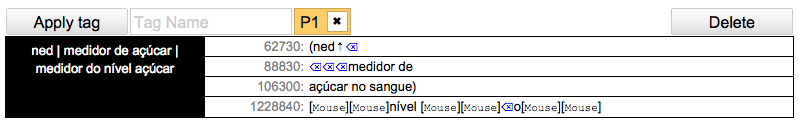
\includegraphics[width=\textwidth]{figures/AlvesF1.png}
\caption{Example of a \isi{macro translation unit} type P1}
\label{fig:alves:1}
\end{figure} 

In Example \ref{ex:alves:2}, two micro units were processed in different phases of the translation process to make up a \isi{macro translation unit}. As shown in \figref{fig:alves:2}, first a micro unit was observed in the drafting phase at 792480ms in a long text segment of 115 characters in which the expression \textit{fora do corpo} `outside the body' appeared. This provisional solution was only revised in the \isi{revision phase}. After a first draft of the \isi{target text} had been produced, at 3596240ms the micro unit was changed into \textit{de forma invasiva} `in an invasive manner' which together with the first rendering makes up a macro unit. Editing within a macro unit which occurs in the \isi{revision phase} is represented by a tilde [ {\Tilde} ]. This type of macro unit was classified as P2, namely a macro unit with processing patterns which occur only once in the drafting phase and are then taken up again during the \isi{revision phase}.

\begin{figure}
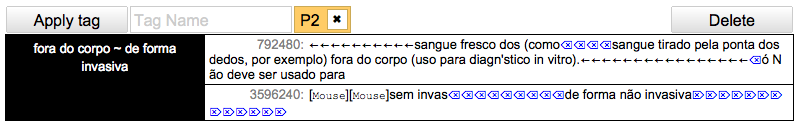
\includegraphics[width=\textwidth]{figures/AlvesF2.png}
\caption{Example of a \isi{macro translation unit} type P2}
\label{fig:alves:2}
\end{figure} 
  
In Example \ref{ex:alves:3}, two micro units occur in the drafting phase as in a P1 type of \isi{macro translation unit}. However, differently from a P1 macro unit, there is also one (or more) micro unit observed in the \isi{revision phase}. As shown in \figref{fig:alves:3}, at 58130ms the micro unit was processed as \textit{medidor de índice} `meter of index'. Next, still in the drafting phase, it was changed into \textit{medidor de glicemis} `meter of blood-sugar-leves /typo/'. Then, at 2108600, during the \isi{revision phase}, the typo ``s'' was deleted and replaced by ``a'' to render \textit{medidor de glicemia} `meter of blood-sugar-level'. This type of macro unit was classified as P3, namely a macro unit with processing patterns which occur more than once in the drafting phase and are taken up again once or more in the \isi{revision phase}.

\begin{figure}
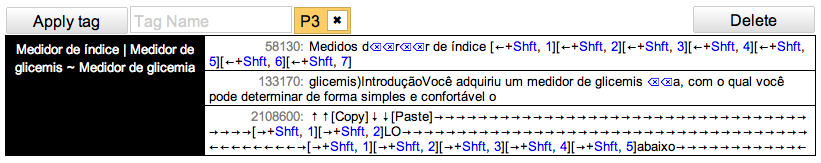
\includegraphics[width=\textwidth]{figures/AlvesF3.png}
\caption{Example of a \isi{macro translation unit} type P3 }
\label{fig:alves:3}
\end{figure} 

In order to carry out the analysis of drafting and revision patterns, XML files with translation process data from the 12 professional translators were segmented into micro units. Each file was then annotaded manually on the basis of the triadic classification, and micro units were classified as P1, P2 and P3. The same procedure was applied to all 12 XML files with translation process data generated by \isi{Translog} 2006. \footnote{For the sake of clarification, we provide a link \url{http://letra.letras.ufmg.br/resources/2010_alves_vale.png} (last accessed 2011-11-24) with access to three appendixes where data analysis is fully displayed. Appendix 1 contains a set of annotated macro units of type P1 whereas Appendix 2 comprises all macro units classified as P2 and Appendix 3 shows the remaining macro units classified as P3.} Using these three categories, all micro units registered in the 12 keylog files with translation process data were annotated as macro units. The next section presents the results of this classification.

\section{Data analysis}\label{sec:alves:4}
In accordance with the proposal made by  \citet{AlvesVale2009} to classify micro and macro translation units, our corpus contains 355 macro units implemented by the 12 subjects. \tabref{tab:alves:1} shows the total number of macro units, made up by a combination of P1, P2 and P3 types.

\begin{table}
\begin{tabular}{lrr}
\lsptoprule

Subject  E1 & \multicolumn{2}{c}{ Number of macro units (P1 + P2 + P3) =}\\
 \midrule 
 E1 & (17 + 21 + 1) = & 39\\
 E2 & (7 + 0 + 0) = &  07\\
 E3 & (9 + 12 + 0) = &  21\\
 E4 &  (29 + 22 + 5) = &  56\\
 E5 &   (4 + 58 + 1) =  & 63\\
 E6 &  (11 + 10 + 0) =  & 21\\
 G1 &   (12 + 29 + 5) = &  46\\
 G2 &   (6 + 5 + 2) =  & 13\\
 G3 &  (23 + 0 + 0) =  & 23\\
 G4 &   (22 + 12 + 2) = &  36\\
 G5 &  (1 + 8 + 0) =  & 09\\
 G6 &  (10 + 10 + 1) =  & 21\\
 \midrule 
 Total &  (151 + 187 + 17) = &  355\\
\lspbottomrule
\end{tabular}
\caption{Total number of macro units per subject}
\label{tab:alves:1}
\end{table} 

By looking at \tabref{tab:alves:1}, one can easily identify a completely different pattern in E5 with 58 occurrences of type P2 and only 4 cases of P1 and 1 case of P3. The next highest count in this category is observed in the performance of G1 with 29 occurences of P2. If we consider E5 as an outlier, the total number of P1 will be 147, with 129 cases of P2 and 16 occurrences of P3, indicating that, on the whole, P1 {\textgreater} P2 {\textgreater} P3. As we have different profiles and different revision total frequencies, the total numbers of P1, P2, and P3 are not informative in themselves. Comparing total P1 and total P2 will result in different rules depending on the profiles we exclude. However, regardless of considering E5 as an outlier or not, P1 and P2 occurrences are far higher than P3 types which makes only 4.8\% of the total number of occurrences in the sample.

\subsection{Identifying patterns of translation units and profiles during drafting and revision}\label{sec:alves:4.1}

\tabref{tab:alves:2} presents the absolute and relative numbers across the sample, separating data among the subjects who translated from English (E1-E6) and from German into Brazilian Portuguese (G1-G6), grouping them according to P1, P2 and P3 types of macro translation units and adding a column with a classification of translator profiles which will be discussed further in this section.


\begin{table}
\resizebox{\textwidth}{!}{
  \begin{tabular}{lllllllll}
  \lsptoprule
   Subject & \multicolumn{2}{l}{ P1} & \multicolumn{2}{l}{ P2} & \multicolumn{2}{l}{ P3} & Profile & Sub-profile\\
  & Abs. & Rel. & Abs. & Rel. & Abs. & { Rel.} &  & \\
  \midrule
   E1 & 17 & 43.7\% & 21 & 53.8\% & 1 & 2.6\% & Drafter/Reviser & Non-Recursive\\
   E2 & 7 & 100\% & 0 & {}-{}-{}-{}- & 0 & {}-{}-{}-{}- & Drafter & \\
   E3 & 9 & 42.9\% & 12 & 57.1\% & 0 & {}-{}-{}-{}- & Drafter/Reviser & Non-Recursive\\
   E4 & 29 & 51.8\% & 22 & 39.2\% & 5 & 8.9\% & Drafter/Reviser & Recursive\\
   E5 & 4 & 6.3\% & 58 & 92.0\% & 1 & 1.6\% & Reviser & \\
   E6 & 11 & 52.4\% & 10 & 47.6\% & 0 & {}-{}-{}-{}- & Drafter/Reviser &   Non-Recursive\\
   G1 & 12 & 26.1\% & 29 & 63.0\% & 5 & 10.9\% & Drafter/Reviser &  Recursive\\
   G2 & 6 & 46.2\% & 5 & 38.5\% & 2 & 15.4\% & Drafter/Reviser &  Recursive\\
   G3 & 23 & 100\% & 0 & {}-{}-{}-{}- & 0 & {}-{}-{}-{}- & Drafter & \\
   G4 & 22 & 61.1\% & 12 & 33.3\% & 2 & 5.6\% & Drafter/Reviser &  Recursive\\
   G5 & 1 & 11.1\% & 8 & 88.9\% & 0 & {}-{}-{}-{}- & Reviser & \\
   G6 & 10 & 47.6\% & 10 & 47.6\% & 1 & 4.8\% & Drafter/Reviser &   Non-Recursive\\
  \lspbottomrule
  \end{tabular}
}
\caption{Absolute and relative numbers for P1, P2 and P3 per subject and corresponding profiles}
\label{tab:alves:2}
\end{table}

If we look at the apparently disparate figures displayed in \tabref{tab:alves:2}, a picture of idiosyncratic patterns might seem to be the first obvious conclusion. However, by closer scrutiny we can identify correlated patterns across the two language pairs. On the one hand, both E2 and G3 only show cases of P1 macro units whereas E5 and G5 display predominant occurrences of P2 macro units. On the other hand, the remaining subjects show a pattern where P1 and P2 types of macro units compete in terms of predominance and sometimes P1 {\textgreater} P2 and at other times P2 {\textgreater} P1. If we apply a formula to the number of occurrences, we can classify the data into four different translator profiles.

A translator was classified with the profile of a ``Drafter'' if, during the drafting phase, he or she revised the TT six times more than during the \isi{revision phase}. Inversely, a translator was classified with the profile of a ``Reviser'' if, during the \isi{revision phase}, he or she revised the TT six times more than during the drafting phase. The remaining translators were classified with the profile of a ``Drafter/Reviser''. Within this group, we found two special subgroups comprised by translators who either revised the same parts of the TT both during the drafting and the revision phases, revisions of the type P3 (Recursive sub-profile) and those who did not (Non-recursive sub-profile). \tabref{tab:alves:3} displays the formulae for calculating the four different profiles.

\begin{table}
\begin{tabular}{ l l }
\lsptoprule
  Drafter &  (P2 + P3) ÷ P1 {\textless} 1/6 \\
  Reviser & P1 ÷ (P2 + P3) {\textless} 1/6  \\
  Drafter Non-Recursive Revise &  (P2 + P3) ÷ P1 ${\geq}$ 1/6 \& P2 ÷ P3 {\textless} 1/6  \\
  Drafter Recursive Reviser & (P2 + P3) ÷ P1 ${\geq}$ 1/6 \& P2 ÷ P3 ${\geq}$ 1/6  \\
  \lspbottomrule
\end{tabular}
\caption{Calculation of translator profiles per types of macro TUs where {\textless} or {\textgreater} 1/6 is a distinctive indicator}
\label{tab:alves:3}
\end{table}

\subsection{Patterns of translator profiles in the drafting and in the revision phases}\label{sec:alves:4.2}

According to our analysis, we identified four types of profiles: Drafters, Re\-visers, Drafter Non-Recursive Revisers, and Drafter Recursive Revisers. Drafters are those subjects who predominantly show P1 types of macro translation units and process them entirely during the drafting phase. Revisers, on the other hand, seem to produce interim solutions in the provisional \isi{target text} while drafting and implementing changes predominantly in the \isi{revision phase}. As far as the third and fourth profiles are concerned, those of the Drafter/Reviser, all subjects had approximately the same number of TT changes in both phases, which can be expressed by 1/2 {\textless} P1 ÷ (P2 + P3) {\textless} 2.

The data analysis shows that neither 1/6 {\textless} (P2 + P3) ÷ P1 {\textless} 1/2 nor 1/6 {\textless} P1 ÷ (P2 + P3) {\textless} 1/2 were observed in the sample. In other words, either the subject had an approximate equal number of changes during the drafting and revision phases or the subject implemented a lot more changes in one phase than in the other. In our corpus, there is no subject with a tendency to revise slightly more in one of the two phases. There are two trends in the sample: a predominant mode of revision either during the drafting or revision phases or a strong tendency towards a balanced distribution of  P1 and P2 types of macro translation units.

When determining the ``Drafter Recursive Reviser'' profile, all translators of the Drafter Reviser profile were found to have approximately six times more changes implemented of type P2 than those of type P3. The ones that are over the threshold of 6 P2s per P3 are on the ``Drafter Non-Recursive Reviser'' profile and the ones who were below this threshold were on the ``Drafter Recursive Reviser'' profile. Again, all translators were close to this threshold. Therefore, these two categories can be understood as slight tendencies in a cline.

At last, by definition, there must be at least one change during the drafting phase for identifying a textual change of the type P3, which can be expressed as P1 {\textgreater} 0 if P3 {\textgreater} 0. Although this is the only rule that must be found by definition, we also found two other rules: in every analysed translation, there were more changes in the drafting phase (P1) than recursive changes in the \isi{revision phase} (P3) and there were always more non-recursive changes in the \isi{revision phase} (P2) than recursive ones (P3), what can be expressed as P1 {\textgreater} P3 and P2 {\textgreater} P3.

\subsection{Patterns of macro translation units in the drafting and in the revision phases}\label{sec:alves:4.3}

 
Besides classifying the data in terms of macro translation units of types P1, P2 and P3 as well as introducing four different translator profiles, the data analysis also allows the observation of subpatterns within the triadic categories. By looking at the data, one observes how decisions previously made by the translator influence the revision patterns in the unfolding of the macro translation units. On the one hand, translation process data such as \isi{key-logging} is linear in time -- one event at a time follows another -- and recursive in the TT: additions, editions and deletions may happen in any position of it. On the other hand, TTs have a linear structure: their characters -- in all their intermediate and final versions -- are organized linearly -- one character after the other. When translating a given micro unit, a choice made at timestamp X may lead the translator to replace a decision made in a previous part of the TT at timestamp Y by an alternative which signals an attempt to standardize choices. This upward movement has been classified as a P1 ascending pattern as shown in \figref{fig:alves:4}.

As displayed in the upper part of \figref{fig:alves:4}, one can see that, as shown at timestamp 471290ms, G4 initially translates the German verb \textit{bestimmen} `determine' into Brazilian Portuguese as \textit{determinar} `determine'. As the process unfolds, two lexical items are translated as \textit{medição} and \textit{medida} `measurement'. Then, as shown at timestamp 557820ms, still in the drafting phase, after translating the noun \textit{Bestimmung} `determination' as \textit{medição} `measurement', G4 changes \textit{determinar} `determine' into \textit{mensurar} `measure'. This upward recursive movement in text production seems to be clearly driven by the lexical choices of \textit{medição/medida} `measurement' and \textit{medição} `measurement' which lead G4 to replace \textit{determinar} by \textit{mensurar}. The upward unfolding of the micro units into a macro unit in the drafting phase illustrates what we call a P1 ascending pattern. 

  
\begin{figure}
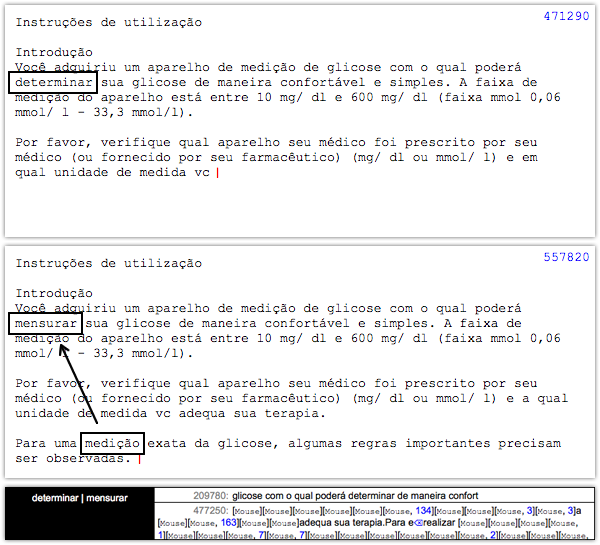
\includegraphics[width=\textwidth]{figures/AlvesF4.png}
\caption{P1 ascending pattern (example of G4 performance)}
\label{fig:alves:4}
\end{figure} 

When translating another given micro unit, a first choice may be replaced by a second alternative which indicates that a previously made decision influences the revision carried out by the translator in an attempt to standardize choices. This downward movement has been classified as a P1 descending pattern as shown in \figref{fig:alves:5}. 


\begin{figure}
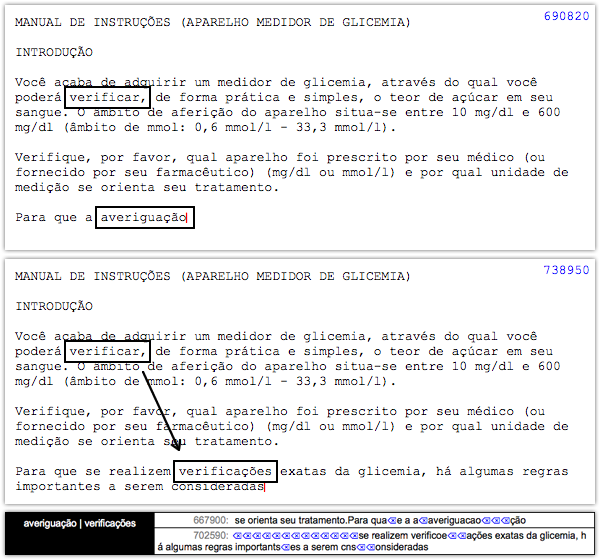
\includegraphics[width=\textwidth]{figures/AlvesF5.png}
\caption{P1 descending pattern (example of G6 performance)}
\label{fig:alves:5}
\end{figure} 

As displayed in the upper part of \figref{fig:alves:5}, one can see that, at timestamp 690820ms, while translating the same source text fragment, G6 initially translates the German verb \textit{bestimmen} `determine' into Brazilian Portuguese as \textit{verificar} `verify'. \figref{fig:alves:5} also shows that \textit{Bestimmungen} `determinations' down below in the same source text fragment was translated as \textit{averiguações} `investigations'. As the process unfolds, at timestamp 738950ms, still in the drafting phase, G6 changes \textit{averiguações} `investigations' into \textit{verificações} `verifications'. This downward recursive movement in text production seems to be clearly driven by the lexical choice of  \textit{verificar} `verify' at shown timestamp 690820ms. The downward unfolding of the micro units into a macro unit in the drafting phase illustrates what we call a P1 descending pattern.

Both ascending and descending subtypes of P1 signal the influence of different stages of text production in the unfolding of macro translation units. What must be clear is that the notion of descending and ascending~movements~is related to but is not the same as the one of previous and following~positions~in the TT. The former are dynamic movements of the subjects over the TT in a process-oriented perspective and the latter are static relative positions of text segments in a product-oriented perspective. Sometimes the driving force is a translation decision made later in the drafting phase which influences the revision of a choice which had already been made earlier in the translation process (P1 ascending pattern). At other times, the driving force is a previously made decision which seems to guide the revision of a translation alternative which is then implemented on the basis of a choice made at a previous timestamp (P1 descending pattern).

Additionally, similar processes of descending types of macro units seem to occur when we move away from the drafting phase. Given our observations of P-types, P2 only shows a descending pattern. In this subtype of \isi{macro translation unit}, a micro unit occurs only once in the drafting phase and is then processed once or more in the \isi{revision phase}.


\begin{figure}[t]
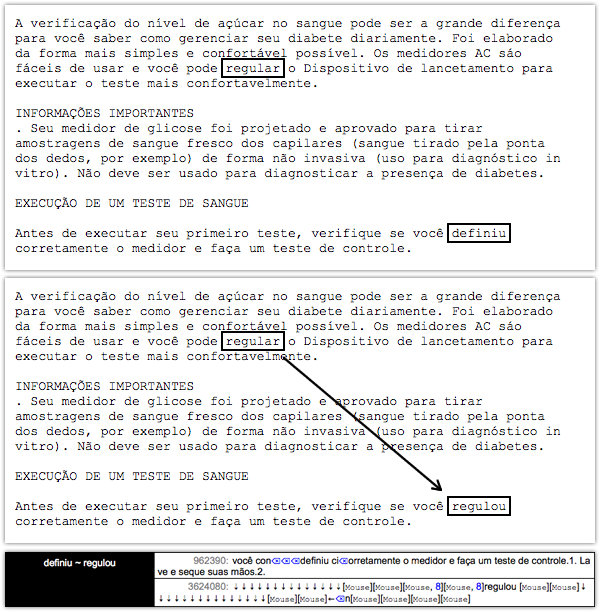
\includegraphics[width=\textwidth]{figures/AlvesF6.png}
\caption{P2 descending pattern (example of E3 performance)}
\label{fig:alves:6}
\end{figure} 

\figref{fig:alves:6} displays an example of a P2 descending pattern. As displayed in the upper part of \figref{fig:alves:6}, one can see that E3 initially translates the pair `adjust' and `set up'  by \textit{regular} `regulate' and \textit{definiu} `defined'. E3 then changes \textit{definiu} `defined' into \textit{regulou} `regulated' during the \isi{revision phase}. The downward unfolding of the micro units into a macro unit in the \isi{revision phase} illustrates what we call a P2 descending pattern.


Finally, as shown in \figref{fig:alves:7}, a descending pattern also seems to be prototypical of P3.


One can see that G6 translates the word set \textit{bestimmen}, \textit{Messbereich}, \textit{Bereich}, \textit{kontrollieren}, \textit{Bestimmungen} by \textit{verificar} `verify', \textit{âmbito de aferição} `scope of verification', \textit{âmbito de aferição} `scope of verification', \textit{verifique} `verify', \textit{verificações} `verifications' and then changes \textit{verificações} `verifications' into \textit{aferições} `verifications' in the \isi{revision phase}. These examples of changes in the \isi{revision phase} show a revision process that is not bound to the lexical correspondences between the source and target languages/texts.


\section{Concluding remarks}\label{sec:alves:5}

The picture emerging from the data analysis is manifold. Using the LITTERAE \isi{annotation} and search tool, it was possible to classify macro translation units according to types P1, P2 and P3. It was also possible to differentiate two main types of macro translation units. On the one hand, P1 can be considered as a type of macro unit which signals online cognitive processing of translation units both in ascending and descending modes. On the other hand, P2 and P3 can be seen as types of macro units which signal a somewhat different process, namely a process that is more detached from the source text and consists of revisions of text production rather than translations per se. This difference is quite striking 
particularly in view of the fact that both P2 and P3 are descending modes of text production in translation. On the whole, P2 types are more frequent than P3 types and more substantial revisions are only found  among P2 types of macro translation units. P3 types seem to account for more fine-grained revisions which are quite small in numbers.

\begin{figure}[t]
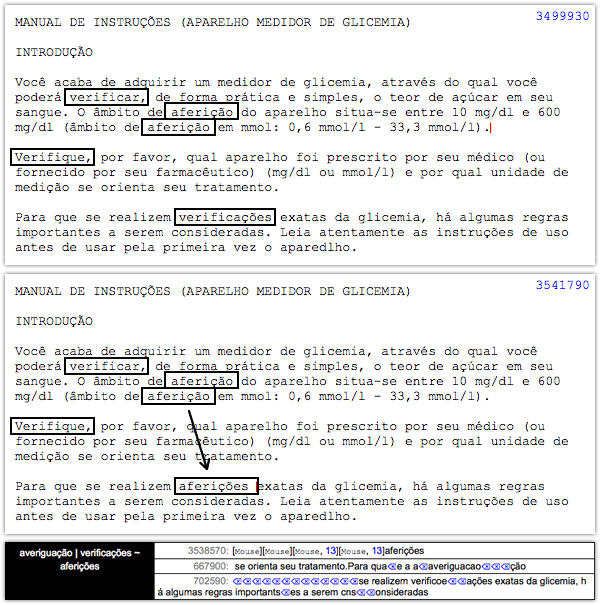
\includegraphics[width=\textwidth]{figures/AlvesF7.png}
\caption{P3 descending pattern (example of G6 performance)}
\label{fig:alves:7}
\end{figure} 

The overall trend shows that in terms of cognitive processing P1 has quite a distinctive nature than that of P2 and P3 and seems to be where translation takes place par excellence. However, the amount of data analysed in this chapter is too small to allow for generalizations. Nevertheless, we hope to have paved the way for future studies by presenting a tool and a methodology which can be replicated and, thus, foster a corpus linguistics oriented analysis of translation process data. 

\section*{Acknowledgements}
\largerpage[-1]
Research developed within the framework of the SEGTRAD Project (Cognitive Segmentation and Translation Memory Systems: investigating the interface between translators' performance and translation technology)  was funded by the Brazilian Research Council (CNPq) grant n° 301270/2005-8.

{\sloppy 
\printbibliography[heading=subbibliography,notkeyword=this]
}
\end{document}

